\documentclass{article}
\usepackage[utf8]{inputenc}
\textheight = 25cm 
\textwidth = 15cm
\topmargin = -2.5cm 
\oddsidemargin = 1.5cm
\usepackage{float}
\usepackage{graphicx}
\graphicspath{{./images/}}

\usepackage{amsmath}
\usepackage{mathtools, xparse}
\usepackage[shortlabels]{enumitem}
\usepackage[most]{tcolorbox}
\usepackage{adjustbox}
\usepackage{bm} 

\DeclarePairedDelimiter{\norm}{\lVert}{\rVert}

\title{Tarea 8 Mecánica Analítica}
\author{Cerritos Lira Carlos}
\date{6 de Mayo del 2020}

\begin{document}
\maketitle
\section*{Problemas}
\section*{1.-}
\subsection*{6.7)}
En un espectrómetro de masas, se acelera un ion posotivo de una sola carga 
($q=1.602 \times 10^{-19} coloumbs$) por medio de una diferencia de potencial de 
$1000 voltios$. Luego pasa por un campo magnético uniforme en el que $B=0.1weber/m^2$,
y se desvía en una trayectoria circular de $0.182m$ de radio. Determinar:
\begin{enumerate}[a)]
    \item La velocidad del ion.
    \item La masa del ion en kilogramos y unidades de masa atómica.
    \item El número de masa del ion.
\end{enumerate}
\begin{tcolorbox}[breakable]
    \subsection*{a)}
    \[v_0 = \frac{2\phi}{qB} = 1.1 \times 10^5 m/seg \]
    \subsection*{b)}
    \[ m = \frac{2T}{v_0^2} = 2.45 \times 10^{-23}g = 14.7uma \]
    \subsection*{c)}
    \[ A = 15 \]
\end{tcolorbox}

\section*{2.-}
\subsection*{6.9}
En la posición $x=0, y=0$, un cañón tiene un alcance máximo $l_m$. Determinar los dos 
ángulos de elevación para hacer blanco en el punto:
\[ x = l_m/2, \quad y=l_m/4 \]
\begin{tcolorbox}[breakable]
    \[ \theta = 45, 75 \]
\end{tcolorbox}

\section*{3.-}
\subsection*{8.13}
Una cuerda de masa $3m$ puede deslizarse horizontalmente sin rozamiento por un alambre 
como se indica en la figura $8-14$. Unido a la cuerda hay un péndulo doble. Si, en una 
posición cercana a la de su equilibrio, se deja el sistema en libertad, a partir del
reposo, las masas oscilan en el plano de la figura a un lado y al otro de la vertical.
\begin{enumerate}[a)]
    \item Escriba las ecuaciones de Lagrange del movimiento del sistema.
    \item Hállese las aceleraciones cuando los desplazamientos y las aceleraciones son pequeñas.
\end{enumerate}
\begin{figure}[H]
    \centering
    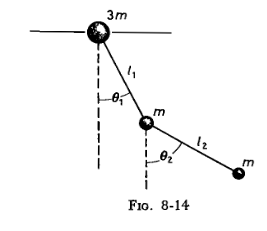
\includegraphics[scale=0.8]{p3_pendulum.png}
\end{figure}
\begin{tcolorbox}[breakable]
    \subsection*{a)}
    \begin{align*}
        T 
        &= \frac{3}{2}m\dot{x}^2 + \frac{1}{2}ml_1^2\dot{\theta}_1^2sin^2\theta_1 + \frac{1}{2}m(l_1 \dot{\theta}_1 cos\theta_1 + \dot{x})^2 \\
        &+ \frac{1}{2}m(l_1\dot{\theta}_1 sin\theta_1 + l_2\dot{\theta}_2 sin\theta_2)^2 \\
        &+ \frac{1}{2}m(l_1\dot{\theta}_1cos\theta_1 + l_2\dot{\theta}_2 cos\theta_2 + \dot{x})^2
    \end{align*}
    \begin{align*}
        U
        &= mgl_1\theta_1^2 + \frac{1}{2}mgl_2\theta_2^2
    \end{align*}
    \subsection*{b)}
    \begin{align*}
        T
        &= \frac{3}{2}m\dot{x}^2 + \frac{1}{2}m(l_1\dot{\theta}_1 + \dot{x})^2 + \frac{1}{2}m(l_1\dot{\theta}_1+l_2\dot{\theta}_2 + \dot{x})^2
    \end{align*}
    \begin{align*}
        U
        &= mgl_1\theta_1^2 + \frac{1}{2}mgl_2\theta_2^2
    \end{align*}

\end{tcolorbox}

\section*{4.-}
\subsection*{Demostración 8.15}
\[ [x_i,l_j] = \sum_{k}e_{ijk}x_k \]
\begin{tcolorbox}[breakable]
    
\end{tcolorbox}

\section*{5.-}
\subsection*{Demostración 8.18}
\[ \frac{\partial }{\partial x}[X,Y] = [\frac{\partial X}{\partial x},Y] + [X,\frac{\partial Y}{\partial x}] \]
\begin{tcolorbox}[breakable]
    
\end{tcolorbox}

\end{document}